%
% Niniejszy plik stanowi przykład formatowania pracy magisterskiej na
% Wydziale MIM UW.  Szkielet użytych poleceń można wykorzystywać do
% woli, np. formatując własna prace.
%
% Zawartość merytoryczna stanowi oryginalnosiagniecie
% naukowosciowe Marcina Wolinskiego.  Wszelkie prawa zastrzeżone.
%
% Copyright (c) 2001 by Marcin Woliński <M.Wolinski@gust.org.pl>
% Poprawki spowodowane zmianami przepisów - Marcin Szczuka, 1.10.2004
% Poprawki spowodowane zmianami przepisow i ujednolicenie
% - Seweryn Karłowicz, 05.05.2006
% Dodanie wielu autorów i tłumaczenia na angielski - Kuba Pochrybniak, 29.11.2016

% dodaj opcję [licencjacka] dla pracy licencjackiej
% dodaj opcję [en] dla wersji angielskiej (mogą być obie: [licencjacka,en])
\documentclass{pracamgr}
\usepackage[hidelinks]{hyperref}
\usepackage{tikz}
% \usepackage{refcheck}
\usepackage{dirtree}
\usepackage{caption}
\usetikzlibrary{shapes,arrows,positioning}

\tikzstyle{decision} = [diamond, draw, fill=blue!20,
    text width=4.5em, text badly centered, node distance=3cm, inner sep=0pt]
\tikzstyle{block} = [rectangle, draw, fill=gray!20,
    text centered, rounded corners, minimum height=4em, minimum width=4cm]
\tikzstyle{line} = [draw, -latex']
\tikzstyle{cloud} = [draw, ellipse,fill=red!20, node distance=3cm,
    minimum height=2em]

% W tym szablonie początki rozdziałów są na nieparzystych stronach, więc pojawia się dużo pustych.
% W wersji "produkcyjnej" trzeba zakomentować.
\let\cleardoublepage\clearpage
\DeclareUnicodeCharacter{00A0}{ }

% blokujemy dzielenie wybranych słów


% Dane magistrantów:
\autor{Dominik Murzynowski}{360180}
\autori{Piotr Zalas}{361374}


\title{Mobilny USOS -- aplikacja mobilna dla studentów i~pracowników uczelni}
%\tytulang{ Mobile USOS - mobile application for university students and employees}

\kierunek{informatyka}

% informatyka - nie okreslamy zakresu (opcja zakomentowana)
% matematyka - zakres moze pozostac nieokreslony,
% a jesli ma byc okreslony dla pracy mgr,
% to przyjmuje jedna z wartosci:
% {metod matematycznych w finansach}
% {metod matematycznych w ubezpieczeniach}
% {matematyki stosowanej}
% {nauczania matematyki}
% Dla pracy licencjackiej mamy natomiast
% mozliwosc wpisania takiej wartosci zakresu:
% {Jednoczesnych Studiow Ekonomiczno--Matematycznych}

% \zakres{Tu wpisac, jesli trzeba, jedna z opcji podanych wyzej}

% Praca wykonana pod kierunkiem:
% (podać tytuł/stopień imię i nazwisko opiekuna
% Instytut
% ew. Wydział ew. Uczelnia (jeżeli nie MIM UW))
\opiekun{dr Janiny Mincer-Daszkiewicz\\
  Wydział Matematyki, Informatyki i Mechaniki\\
  }

% miesiąc i~rok:
\date{Czerwiec 2019}

%Podać dziedzinę wg klasyfikacji Socrates-Erasmus:
\dziedzina{
%11.0 Matematyka, Informatyka:\\
%11.1 Matematyka\\
%11.2 Statystyka\\
11.3 Informatyka\\
%11.4 Sztuczna inteligencja\\
%11.5 Nauki aktuarialne\\
%11.9 Inne nauki matematyczne i informatyczne
}

%Klasyfikacja tematyczna wedlug AMS (matematyka) lub ACM (informatyka)
\klasyfikacja{Software and its engineering\\
	Software creation and management\\
	Designing software\\
	Software implementation planning\\
	Software design techniques}

% Słowa kluczowe:
\keywords{USOS, Android, Kotlin}

% Tu jest dobre miejsce na Twoje własne makra i~środowiska:
\newtheorem{defi}{Definicja}[section]
\usepackage{url}
\usepackage{booktabs}
\usepackage{graphicx}
\usepackage{tabu}
\usepackage{caption}

% reguły łamania słów
\hyphenation{USOS-web}
\hyphenation{USOS-mail}
\hyphenation{USOS-adm}
\hyphenation{USOS}
\hyphenation{MUCI}

% koniec definicji
\usepackage{tocloft}
\setlength{\cftchapnumwidth}{1.75em}
\usepackage[acronym, numberedsection]{glossaries}

\makeglossaries

% Nowe obiekty do slownika:
%\newglossaryentry{Luminis}
%{
%    name=Luminis,
%    description={Aplikacja WWW wizualizująca stan lamp ulicznych w czasie rzeczywistym, korzystając z technologii służących do przechowywania szeregów czasowych}
%}


\begin{document}

\maketitle
%tu idzie streszczenie na stronę początkową
\begin{abstract}
  W ramach pracy powstała aplikacja mobilna dla
  studentów i~pracowników. Aplikacja daje dostęp do najczęściej wykorzystywanych 
  funkcjonalności USOSweb. Nie powiela wszystkiego, co dostępne w~serwisie 
  webowym, ale umożliwia wygodny dostęp do tych informacji 
  i~funkcjonalności, do których student czy 
  pracownik chce sięgać w~dowolnym miejscu i~czasie, bezpośrednio ze swojego smartfona. 
  W~ramach pracy zostały zaimplementowane m.in. moduły do obsługi 
  sprawdzianów i~ocen, zarówno po stronie studenta, jak i~pracownika, katalogi
  przedmiotów i~osób oraz~plan zajęć. Ważną usługą zapewnianą przez 
  aplikację jest powiadamianie o~zdarzeniach w~czasie rzeczywistym, typu wystawione
  oceny. Aplikacja została wdrożona na UW i~kilkunastu innych uczelniach, projekt zakłada możliwość udostępnienia
  aplikacji wszystkim uczelniom korzystającym z~USOS. Do aplikacji dołączyliśmy
  dokumentację instalacyjną dla wdrożeniowców.
  Aplikacja będzie dostępna na platformie Android.
\end{abstract}

\tableofcontents
%\listoffigures
%\listoftables

\setlength{\LTpost}{0pt} % Lepsze marginesy w longtable

\chapter{Wstęp}

Mobilny USOS powstaje w~ramach projektu ,,e-UW – rozwój e-usług Uniwersytetu Warszawskiego
związanych z~edukacją'', realizowanego w~latach 2016-2019 \cite{euslugi}.

Proces tworzenia aplikacji rozpoczął się w~roku 2016. Autorami kodu w~pierwszej iteracji
rozwoju byli programiści z~Uniwersytetu Łódzkiego. Zakończyli oni prace nad kodem
w~styczniu 2018~r. Na tym etapie prac aplikacja miała moduły: aktualności, ankiety, oceny,
informacje o~uczelni, dashboard, mapa, plan zajęć oraz katalog osób i~zajęć (nazywany
wtedy modułem dziekanatu). Aplikacja od początku była rozwijana w~językach polskim
i~angielskim, analogicznie do innych modułów systemu USOS, jak USOSweb.

Od kwietnia 2018~r. przejęliśmy rozwój aplikacji. Naszym głównym celem
było wdrożenie na uczelniach z~konsorcjum MUCI. MUCI -- Międzyuniwersyteckie Centrum Informatyzacji --  zajmuje się m.in. tworzeniem, rozwojem i~wdrażaniem systemów wspierających
uczelnie \cite{muci}. W~ramach dążenia do tego celu naszymi zadaniami
były m.in. refaktoring kodu, rozbudowa o~nowe moduły oraz dostosowanie do potrzeb osób 
niepełnosprawnych.

Istotnym elementem refaktoringu kodu była migracja z~Javy na Kotlin (o~wyborze technologii obecnych w~produkcyjnej wersji
aplikacji opowiemy w~rozdziale 4.), zastąpienie wadliwego rozwiązania problemu
wykonywania asynchronicznych zapytań do USOS API przez mechanizm korutyn 
(ang. \textit{coroutines}) oraz naprawienie innych błędów w~oryginalnym kodzie.

1 października 2018 roku wdrożyliśmy oficjalnie Mobilnego USOS na Uniwersytecie Warszawskim,
wypełniając tym samym pierwszą część celu pracy -- wdrożenie produkcyjne pierwszej uczelni.
W~rozdziale 7. wskażemy wyzwania związane z~procesem wdrażania oraz procedury wdrożeniowe.

Równolegle do prac nad wdrażaniem aplikacji na kolejnych uczelniach rozwijaliśmy kolejne
moduły w~ramach strategii ciągłego rozwoju. W~rozdziale 6. przedstawimy przegląd
funkcjonalności aplikacji.

W~pracy przedstawimy także proces projektowania i~rozwijania aplikacji -- w~rozdziale 2.
wizję projektu, w~3. specyfikację wymagań, w~5. szczegóły implementacji.

% We wstępie Słownik pojęć, Co to właściwie jest, opis firmy, czemu wybraliśmy ten projekt,(?wizja?)
%Przedstawienie problemu
%Przedstawienie produktu
%Opis użytkowników i ich cele
%Funkcje programu
%Licencja
%Wykorzystane technologie

\chapter{Wizja}

\section{Aplikacje mobilne na innych uczelniach}

Na zlecenie Międzyuniwersyteckiego Centrum Informatyzacji \cite{muci} przeprowadzono
badania na temat wykorzystania aplikacji mobilnych przez uczelnie w~Polsce i~na świecie. W~wyniku tych badań ustalono, że aplikacje mobilne
cieszą się dużą popularnością wśród studentów i~pracowników uczelni, ale
między polskimi i~zagranicznymi uczelniami występują duże rozbieżności w~pojmowaniu roli tych aplikacji.

W~Polsce dominuje myślenie, że aplikacja mobilna dla uczelni ma służyć głównie
wymianie informacji pomiędzy studentami, nauczycielami akademickimi i~administracją
uczelni. Systemy informatycznie mają usprawniać formalne procesy, takie jak
wystawianie ocen, informowanie o~wynikach kolokwium, czy dostarczanie 
planu zajęć. Zamieszczone treści i~komunikaty napisane są językiem wskazującym na
urzędowy charakter relacji pomiędzy użytkownikami systemu.

W~przypadku uczelni zagranicznych aplikacje mobilne mają mniej formalny
charakter. Oprócz usprawniania komunikacji między studentami, nauczycielami
akademickimi i~pracownikami administracji pełnią także funkcję społecznościową.
Organizacje studenckie tych uczelni mają swoje wydzielone miejsce w~aplikacji
mobilnej, gdzie mogą się promować, informować o~ciekawych wydarzeniach i~spotkaniach
mających miejsce w~obrębie uczelnianego kampusu. Sama szata graficzna tych części
aplikacji jest mniej surowa, a~edytorzy treści pozwalają sobie na
swobodniejszy dobór grafik i~użycie nieformalnego języka. 

Mobilny USOS ma być uzupełnieniem USOSweb, przewidujemy dla niego rolę informacyjną,
zgodną z~dominującym w~Polsce podejściem do tematu aplikacji mobilnej dla uczelni,
bez aspektu społecznościowego.

\section{Aplikacja mobilna dla USOS}

Na bazie wniosków z przeprowadzonego badania zdecydowano, że Uniwersytecki
System Obsługi Studiów \cite{usos} także ma mieć aplikację mobilną. Możliwe były dwa
modele dostępu do danych zgromadzonych w~USOS:

\begin{itemize}
	\item USOSweb w~wersji na smartfony i~tablety.
	\item Natywna aplikacja mobilna pobierająca dane z~USOS poprzez USOS API \cite{usosapi}.
\end{itemize}

Realizacja pierwszego wariantu wydawała się być bardziej atrakcyjna z~finansowego
punktu widzenia, gdyż nie trzeba by było wtedy tworzyć nowej aplikacji, a~tylko
dostosować USOSweb do potrzeb aplikacji mobilnych. Niestety ze względu na architekturę
USOSweb i~naleciałości historyczne zadanie to okazało się być technicznie niewykonalne
w realistycznym horyzoncie czasowym. Ponadto taka realizacja aplikacji mobilnej
pozbawia użytkownika wielu benefitów wypływających z~natywnej implementacji.
W nowej aplikacji wiele funkcjonalności USOSweb może być dostarczanych w~inny
sposób, który jest dostosowany do specyfiki urządzeń mobilnych.

W związku z~przytoczonymi argumentami MUCI podjęło decyzję o~stworzeniu natywnej
aplikacji Mobilny USOS dla platformy Android. Oczywiście Mobilny USOS z~założenia
nie ma reimplementować całej funkcjonalności USOSweb, tylko jego najważniejsze
moduły w~wersji dostosowanej do charakteru aplikacji mobilnej.
Aby wyłonić kluczowe dla studenta moduły, postanowiono przeprowadzić
ogólną ankietę wśród studentów Uniwersytetu Mikołaja Kopernika w~Toruniu (UMK) i~Uniwersytetu
Śląskiego (UŚ), oraz nieco bardziej szczegółową ankietę wśród studentów i~samorządu
Wydziału Matematyki, Informatyki i~Mechaniki Uniwersytetu Warszawskiego (MIM UW).

\section{Wyniki ogólnej ankiety przeprowadzonej na UMK i UŚ}

Na początku ankiety poproszono respondentów o~podanie podstawowych informacji o~stopniu studiów i~trybie studiowania. Ankietę wypełniło 1216 studentów UMK i~703 studentów UŚ.

\begingroup
\centering
\begin{longtabu} to \textwidth { |X[l]|X[l]|X[l]| }
	\hline
	Odpowiedź & Liczba studentów UMK, którzy zaznaczyli daną odpowiedź & Liczba studentów UŚ, którzy zaznaczyli daną odpowiedź\\
	
	\hline
	\multicolumn{3}{|c|}{\textbf{Wskaż stopień swoich studiów}} \\
	\hline
	
	Pierwszego stopnia & 708 & 366\\
	Drugiego stopnia & 303 & 159\\
	Jednolite magisterskie & 189 & 163\\
	Trzeciego stopnia & 43 & 23\\
	Podyplomowe & 8 & 1\\
		
	\hline
	\multicolumn{3}{|c|}{\textbf{Wskaż tryb swoich studiów}} \\
	\hline

	Stacjonarne & 1142 & 606\\
	Niestacjonarne - wieczorowe & 8 & 14\\
	Niestacjonarne - zaoczne & 73 & 90\\
	\hline
\end{longtabu}
\captionof{table}{Stopień i~tryb studiowania u ankietowanych studentów UMK i~UŚ}\label{tbl:studank}
\medskip
\endgroup

Następnie spytano ankietowane osoby, jak często korzystają z~wymienionych modułów USOSweb.

\begingroup
\centering
\begin{longtabu} to \textwidth { |X[l]|X[l]|X[l]| }
	\hline
	Częstotliwość & Liczba studentów UMK, którzy zaznaczyli daną odpowiedź & Liczba studentów UŚ, którzy zaznaczyli daną odpowiedź\\
	
	\hline
	\multicolumn{3}{|c|}{\textbf{Katalog studentów, pracowników, przedmiotów, kierunków studiów}} \\
	\hline
	
	Codziennie & 309 & 42\\
	Raz w~tygodniu & 361 & 187\\
	Raz na miesiąc & 332 & 195\\
	Raz na semestr & 134 & 150\\
	Raz na rok & 17 & 25\\
	Jednorazowo & 51 & 59\\
	Nigdy & 12 & 45\\
	
	\hline
	\multicolumn{3}{|c|}{\textbf{Plan zajęć}} \\
	\hline
	Codziennie & 428 & 83\\
	Raz w~tygodniu & 459 & 126\\
	Raz na miesiąc & 133 & 95\\
	Raz na semestr & 84 & 75\\
	Raz na rok & 5 & 9\\
	Jednorazowo & 31 & 62\\
	Nigdy & 74 & 253\\
	
	\hline
	\multicolumn{3}{|c|}{\textbf{USOSmail (formularz poczty elektronicznej)}} \\
	\hline
	Codziennie & 847 & 18\\
	Raz w~tygodniu & 205 & 36\\
	Raz na miesiąc & 62 & 57\\
	Raz na semestr & 17 & 47\\
	Raz na rok & 9 & 19\\
	Jednorazowo & 27 & 84\\
	Nigdy & 49 & 442\\	
	
	\hline
	\multicolumn{3}{|c|}{\textbf{Rejestracje na przedmioty, zajęcia, egzaminy}} \\
	\hline
	Codziennie & 17 & 12\\
	Raz w~tygodniu & 61 & 21\\
	Raz na miesiąc & 117 & 56\\
	Raz na semestr & 957 & 523\\
	Raz na rok & 19 & 19\\
	Jednorazowo & 34 & 33\\
	Nigdy & 11 & 37\\
	
	\hline
	\multicolumn{3}{|c|}{\textbf{Sprawdziany}} \\
	\hline
	Codziennie & 65 & 19\\
	Raz w~tygodniu & 137 & 55\\
	Raz na miesiąc & 159 & 61\\
	Raz na semestr & 167 & 88\\
	Raz na rok & 36 & 6\\
	Jednorazowo & 110 & 46\\
	Nigdy & 538 & 428\\
	
	\hline
	\multicolumn{3}{|c|}{\textbf{Oceny}} \\
	\hline
	Codziennie & 368 & 76\\
	Raz w~tygodniu & 350 & 119\\
	Raz na miesiąc & 273 & 164\\
	Raz na semestr & 202 & 261\\
	Raz na rok & 5 & 5\\
	Jednorazowo & 15 & 30\\
	Nigdy & 3 & 48\\
	
	\hline
	\multicolumn{3}{|c|}{\textbf{Podpięcia przedmiotów pod programy studiów}} \\
	\hline
	Codziennie & 10 & 9\\
	Raz w~tygodniu & 40 & 17\\
	Raz na miesiąc & 98 & 61\\
	Raz na semestr & 900 & 324\\
	Raz na rok & 27 & 16\\
	Jednorazowo & 88 & 66\\
	Nigdy & 52 & 207\\
	
	\hline
	\multicolumn{3}{|c|}{\textbf{Podania studenckie}} \\
	\hline
	Codziennie & 7 & 6\\
	Raz w~tygodniu & 15 & 11\\
	Raz na miesiąc & 90 & 32\\
	Raz na semestr & 323 & 143\\
	Raz na rok & 144 & 38\\
	Jednorazowo & 265 & 115\\
	Nigdy & 372 & 355\\
	
	\hline
	\multicolumn{3}{|c|}{\textbf{Wnioski (o stypendia naukowe i~socjalne, akademik, zapomogę itp.)}} \\
	\hline
	Codziennie & 9 & 4\\
	Raz w~tygodniu & 12 & 15\\
	Raz na miesiąc & 84 & 51\\
	Raz na semestr & 263 & 157\\
	Raz na rok & 293 & 62\\
	Jednorazowo & 184 & 91\\
	Nigdy & 370 & 319\\
	
	\hline
	\multicolumn{3}{|c|}{\textbf{Międzynarodowa wymiana studencka}} \\
	\hline
	Codziennie & 4 & 4\\
	Raz w~tygodniu & 4 & 4\\
	Raz na miesiąc & 24 & 6\\
	Raz na semestr & 66 & 14\\
	Raz na rok & 49 & 14\\
	Jednorazowo & 102 & 43\\
	Nigdy & 966 & 615\\
	
	\hline
	\multicolumn{3}{|c|}{\textbf{Ankiety}} \\
	\hline
	Codziennie & 5 & 6\\
	Raz w~tygodniu & 33 & 16\\
	Raz na miesiąc & 105 & 110\\
	Raz na semestr & 567 & 178\\
	Raz na rok & 95 & 58\\
	Jednorazowo & 234 & 215\\
	Nigdy & 177 & 116\\
	
	\hline
	\multicolumn{3}{|c|}{\textbf{Płatności}} \\
	\hline
	Codziennie & 5 & 4\\
	Raz w~tygodniu & 19 & 7\\
	Raz na miesiąc & 159 & 50\\
	Raz na semestr & 162 & 119\\
	Raz na rok & 101 & 63\\
	Jednorazowo & 324 & 189\\
	Nigdy & 446 & 269\\
	
	\hline
\end{longtabu}
\captionof{table}{Jak często studenci UMK i~UŚ korzystają z~poszczególnych modułów USOSweb}\label{tbl:usoswebank}
\medskip
\endgroup

Następnie zapytano o~sprawy związane z~aplikacją mobilną.

\begingroup
\centering
\begin{longtabu} to \textwidth { |X[l]|X[l]|X[l]| }
	\hline
	Odpowiedź & Liczba studentów UMK, którzy zaznaczyli daną odpowiedź & Liczba studentów UŚ, którzy zaznaczyli daną odpowiedź\\
	
	\hline
	\multicolumn{3}{|p{\dimexpr 3\tabucolX+3\tabcolsep+\arrayrulewidth\relax}|}{\textbf{Czy Twoim zdaniem przydatna byłaby aplikacja na urządzenia mobilne oferująca funkcje serwisu USOSweb?}} \\
	\hline
	
	Tak & 1172 & 590\\
	Nie & 43 & 109\\
	
	\hline
	\multicolumn{3}{|p{\dimexpr 3\tabucolX+3\tabcolsep+\arrayrulewidth\relax}|}{\textbf{Jakie moduły serwisu USOSweb powinny być obsługiwane w~takiej aplikacji?}} \\
	\hline
	
	Katalogi & 832 & 394\\
	Plan zajęć & 1127 & 515\\
	USOSmail & 1087 & 181\\
	Rejestracje & 726 & 530\\
	Sprawdziany & 410 & 268\\
	Oceny & 1179 & 624\\
	Podpięcia & 459 & 237\\
	Podania studenckie & 248 & 177\\
	Wnioski & 355 & 259\\
	Międzynarodowa wymiana studencka & 126 & 75\\
	Ankiety & 267 & 94\\
	Płatności & 310 & 220\\
	Inne & 25 & 13\\
	
	\hline
	\multicolumn{3}{|p{\dimexpr 3\tabucolX+3\tabcolsep+\arrayrulewidth\relax}|}{\textbf{Jakie systemy operacyjne posiadasz w~swoich urządzeniach mobilnych?}} \\
	\hline
	
	Android & 1028 & 540\\
	iOS & 189 & 90\\
	Windows Phone & 201 & 113\\
	Inne & 22 & 23\\
	Nie wiem & 21 & 34\\
	Nie posiadam urządzenia mobilnego & 15 & 27\\
	
	\hline
\end{longtabu}
\captionof{table}{Pytania o~aplikację mobilną do ankietowanych studentów UMK i~UŚ}\label{tbl:mobilank}
\medskip
\endgroup

Z przeprowadzonej ankiety wyciągneliśmy następujące wnioski:
\begin{itemize}
	\item Zdecydowana większość studentów uważa, że aplikacja mobilna oferująca funkcje serwisu USOSweb byłaby przydatna.
	\item Moduły, które przynajmniej 50\% studentów obu uczelni chciałoby widzieć w~Mobilnym USOS to: Katalogi, Plan zajęć, Rejestracje, Oceny.
	\item Kolejnymi często wskazywanymi modułami są: Sprawdziany, Podpięcia, Wnioski, Płatności.
	\item Wśród studentów UMK najczęściej wykorzystywanym modułem USOSweb jest USOSmail. Jest to drugi w~kolejności najważniejszy moduł wskazany przez studentów tej uczelni do realizacji w~Mobilnym USOS. Co zaskakujące, u studentów UŚ ten moduł spotkał się z~bardzo niskim zainteresowaniem.
	\item Najniższym zainteresowaniem cieszy się moduł międzynarodowej wymiany akademickiej. Blisko końca listy znalazły się też ankiety i~podania studenckie.
	\item Wśród modułów niewymienionych w~ankiecie studenci zazwyczaj wskazywali na stypendia.
	\item Dominującym systemem operacyjnym w~urządzeniach mobilnych studentów jest system Android. Windows Phone i~iOS znalazły się w~zdecydowanej mniejszości.
\end{itemize}

\section{Wyniki ankiety wśród studentów i~samorządu Wydziału MIM UW}

Studenci Wydziału MIM UW wypełniający ankietę wskazali następujące moduły, które
chcieliby znaleźć w~Mobilnym USOS:

\begin{itemize}
	\item Przeglądarkę ocen i~sprawdzianów.
	\item Plan zajęć wraz z~powiadamianiem o~zbliżających się zajęciach
	      i~kolokwiach.
	\item Katalogi wraz z~wyszukiwarkami.
	\item Mapę uniwersytetu z~podziałem na poszczególne wydziały, wraz z
	      możliwością nawigowania do wybranej lokalizacji.
	\item Rejestracje na zajęcia.
	\item Podpięcia.
\end{itemize}

Do tej listy samorząd studencki Wydziału MIM UW dopisał:

\begin{itemize}
	\item Informacje o~wydziale przydatne dla studenta -- godziny otwarcia sekcji
	      studenckiej, terminy dyżuru dziekana wraz z~elektronicznymi zapisami na
	      dyżur, aktualny plan sesji.
	\item Wypełnianie ankiet wraz z~powiadomieniami o~nowych ankietach.
	\item Decyzje i~statusy podań.
	\item Kalendarz rejestracji wraz z~powiadomieniami.
	\item Synchronizację kalendarza widocznego w~USOSweb z~kalendarzem telefonu.
\end{itemize}
Samorząd wyraził też obawę, że aplikacja mająca za dużo funkcji, niekoniecznie
użytecznych dla większości studentów, będzie mniej przyjazna w~obsłudze.

W wyniku przeprowadzonych ankiet przyjęto do realizacji następujące moduły:
ankiety, katalog, oceny, plan zajęć, sprawdziany, przydatne informacje o~uczelni.

\section{Oczekiwania nauczycieli akademickich i administracji uczelni}

Logika USOS związana z~pracownikami jest bez porównania znacznie bardziej
skomplikowana od logiki związanej ze studentami. Nie ma sensu przepisywać do
aplikacji mobilnej modułów związanych np. z~uzupełnianiem sylabusów, gdyż
nie dość, że takie moduły są używane stosunkowo rzadko, to jeszcze operacje
z ich użyciem wykonuje się zdecydowanie wygodniej z~poziomu komputera. Postanowiliśmy
zaimplementować tylko te moduły, które byłyby przydatne w~sytuacji kiedy pracownik
nie ma dostępu do komputera, np. w~trakcie zajęć lub kiedy nadgorliwy student
spotka pracownika na korytarzu swojego wydziału i~będzie oczekiwał natychmiastowej
informacji na temat swojej oceny.

W związku z~powyższym, do realizacji przyjęliśmy moduł ankiet, protokołów
egzaminacyjnych i~część funkcjonalności sprawdzianów związanej z~wystawianiem
punktów i~ocen. Moduł ankiet jest o~tyle istotny, że władzom uczelni zależy na
zwiększeniu liczby wypełnianych ankiet. Kolejnym modułem, niezwykle ważnym z~punktu widzenia biura prasowego uczelni, są aktualności, które pozwalają pracownikom
biura publikować artykuły wyświetlane w~Mobilnym USOS.

Przy projektowaniu aplikacji należy uwzględnić różnice między uczelniami.
Przykładowo, każda uczelnia we własnym zakresie wdraża nowe wersje USOS API.
Ponadto uczelnie mają wdrożone swoje własne standardy identyfikacji wizualnej.
Należy zapewnić uczelniom możliwość personalizacji wybranych elementów szaty
graficznej Mobilnego USOS. Przy wdrażaniu aplikacji należy pamiętać o~sprawdzeniu kompatybilności z~zainstalowaną przez uczelnię wersją serwera USOS API.
Z wymienionych powodów zdecydowano, że każda uczelnia będzie miała własną
wersję Mobilnego USOS tworzoną ze wspólnego szablonu. W~związku z~faktem, że
niektóre uczelnie nie korzystają z~części funkcjonalności USOSweb (na przykład nie
wpisują do USOS planów zajęć), udostępniliśmy możliwość ukrycia wybranych modułów aplikacji,
tak by uniknąć negatywnych komentarzy użytkowników końcowych związanych z~pustymi zakładkami.

Największe polskie uczelnie są instytucjami publicznymi i~muszą spełniać wytyczne
dostępności narzucane przez polskie prawo \cite{uodc}. W~przypadku aplikacji mobilnych
największy nacisk położony jest na spełnienie norm dotyczących kontrastu i~prawidłowe
współdziałanie z~oprogramowaniem wspierającym osoby niewidome, takim jak Google
TalkBack \cite{talkback}.

\chapter{Specyfikacja wymagań}

\section{Logowanie do aplikacji}

Mobilny USOS, jako część aplikacji rozwijanych w~ramach USOS, powinien być silnie 
zintegrowany z~całą platformą. Logowanie do aplikacji powinno być bezpieczne i~możliwie
intuicyjne dla użytkowników końcowych.

Postulowaną przez przedstawicieli niektórych uczelni i~przez twórców USOS API
metodą przeprowadzenia procesu uwierzytelniania było otwieranie standardowego ekranu
logowania do USOS, a~następnie, po udanym potwierdzeniu tożsamości użytkownika
i~nadaniu uprawnień do aplikacji, powrót do tejże.

Dodatkowo, w~przeciwieństwie do na przykład USOSweb, aplikacja powinna utrzymywać
sesję użytkownika bezterminowo, do wylogowania się bądź odinstalowania aplikacji.
Pozwala to uniknąć regularnego wpisywania hasła, co na telefonie jest szczególnie
niewygodne, a~także niebezpieczne, ponieważ atakujący może łatwiej podejrzeć hasło.

Ostatnim z~wymagań z~zakresu logowania i~bezpieczeństwa było zabezpieczenie aplikacji
przed wykorzystaniem aktywnej sesji przez niepowołane osoby. Wymaganie to zostało później
sprecyzowane -- użytkownik powinien móc wskazać, że aplikacja przy każdym uruchomieniu
ma zażądać hasła do odblokowania.

\section{Dashboard}

Głównym ekranem i~sercem aplikacji jest dashboard. W~zależności od punktu widzenia, pełni
on kilka ról.

Z~punktu widzenia studenta i~pracownika, ważna jest możliwość szybkiego sprawdzenia informacji
potrzebnych w~ciągu dnia na uczelni. Oczywistym przykładem takiej informacji jest plan zajęć,
który także wyświetla się na ekranie głównym USOSweb zarówno u pracownika, jak i~u~studenta.
Student ponadto powinien otrzymywać szybką informację o~nowych ocenach i~wynikach sprawdzianów.

Z~punktu widzenia uczelni, ważna są ankiety i~przekazywanie na bieżąco aktualności z~życia
uczelni.Uczelnie chcą zmaksymalizować liczbę
wypełnionych ankiet i~dzięki temu ulepszać swoją ofertę programową i~lepiej dobierać
prowadzących przedmioty. Prowadzący otrzymują przez ankiety przydatną informację zwrotną.
Dlatego podczas sesji ankietowej w~dashboardzie powinna wyświetlać się lista aktywnych
ankiet, czekających na wypełnienie. Wyświetlanie aktualności w~aplikacji ma na
celu zwiększenie zainteresowania tym,
co ogólnie dzieje się na uczelni. Dzięki aplikacji, artykuły znacznie zwiększą swój zasięg,
ponieważ student lub pracownik, którzy do tej pory nie zaglądali na portal z~wiadomościami
o~uczelni, dowiedzą się o~samym fakcie istnienia tych wiadomości, a~od tego dość blisko do
ich przeczytania, jeśli nagłówek będzie interesujący.

\section{Oceny}

Do modułów aplikacji najbardziej pożądanych przez studentów zdecydowanie należą oceny.
Możemy na ten moduł spojrzeć z~dwóch perspektyw2 -- studenta i~pracownika.

Z~perspektywy studenta możemy wskazać dwie najważniejsze funkcjonalności. Pierwsza to
informacja o~nowych ocenach. Studenci wskazywali, że ważnym sposobem informowania o~nowej
ocenie jest powiadomienie systemowe w~momencie wystawienia oceny, tak by student natychmiast
wiedział, że taka ocena się pojawiła. Dodatkowo, o~nowych ocenach powinien być powiadamiany
w~dashboardzie. Drugą funkcjonalnością jest podgląd wszystkich otrzymanych do tej pory ocen,
analogicznie jak w~USOSweb, tak aby logowanie to systemu przeglądarkowego nie było konieczne.

Z~perspektywy pracownika przydatną funkcjonalnością jest wpisywanie ocen do protokołów
oraz późniejszy podgląd i~edycja już wystawionych. USOSweb udostępnia tę funkcjonalność
w~trzech wariantach:
\begin{itemize}
	\item ,,wystaw szybko ocenę'', gdzie wyszukawszy studenta po imieniu i~nazwisku bądź
	numerze indeksu, pracownik otrzymuje listę protokołów, w~których może wystawić ocenę
	studentowi,
	\item widok listy wszystkich dostępnych protokołów, gdzie po wybraniu jednego
	z~nich pojawia się lista osób, którym w~ramach tego protokołu można wystawić ocenę,
	\item możliwość automatycznego przepisania oceny ze sprawdzianów.
\end{itemize}

Ze względu na przewidywane przypadki użycia Mobilnego USOS przez pracowników --
wystawianie oceny z~jednego przedmiotu kolejnym egzaminowanym ustnie studentom
i~odpowiedzi na pytania studentów o~ocenę, najbardziej przydatnym i~wygodnym wydało się
udostępnienie w~aplikacji mobilnej wariantu drugiego protokołów. Nacisk tu należy położyć na
przejrzystość interfejsu i~umożliwienie edycji wszystkich elementów wpisu do protokołu
(samej oceny, ale także komentarza publicznego, widocznego dla studenta i~prywatnego,
dostępnego tylko dla pracownika w~widoku protokołu).

\section{Sprawdziany}

Na niektórych uczelniach i~wydziałach (chociażby na Wydziale MIM UW, czy na Politechnice
Warszawskiej) intensywnie korzysta się z~modułu sprawdzianów. Przedstawiciele tych
uczelni zabiegali o~wprowadzenie do Mobilnego USOS obsługi sprawdzianów.
Podobnie do przypadku ocen, na moduł możemy spojrzeć z~perspektywy studenta i~pracownika.

Ze względu na fakt, że potrzeby studenta są analogiczne, jak w~przypadku ocen -- powiadomienia
o~nowych punktach i~ocenach w~sprawdzianach oraz dostęp do informacji o~wszystkich wpisach
w~sprawdzianach, nie będziemy tu opisywać wymagań bardziej szczegółowo. Istotną różnicą
w~stosunku do ocen jest dostęp do histogramów wyników, dzięki czemu studenci w~trakcie
roku mogą porównywać swoje wyniki z~ogółem studentów, na przykład aby przewidywać, jakie
mogą być progi punktowe na koniec semestru.

Z~perspektywy pracownika, oczekiwane funkcjonalności aplikacji mobilnej różnią się od tego,
co jest dostępne w~USOSweb. Mając na uwadze wygodę użytkowania, zdecydowano
o~ograniczeniu funkcjonalności do wystawiania punktów, ocen i~możliwości pokazania bądź
ukrycia wyników danego węzła w~drzewie sprawdzianu. Zrezygnowano ze zbyt skomplikowanego
widoku edycji struktury drzewa, algorytmu automatycznego wystawiania oceny oraz z~przepisywania
oceny do protokołu.

\section{Kalendarz roku akademickiego}

Politechnika Warszawska zgłosiła chęć pokazania użytkownikom kalendarza wydarzeń
roku akademickiego. Moduł ten ma powstać w~oparciu o~funkcjonujący w~systemie USOS
kalendarz, który służy np. do obliczania, które dni są wolne od zajęć dydaktycznych
czy jak wygląda podział semestru na tygodnie parzyste i~nieparzyste. Widok w~aplikacji
miał stanowić naturalne rozwinięcie istniejącego raportu, który jednostka może wygenerować
z~systemu administracyjnego USOSadm.

W~widoku użytkownik powinien mieć możliwość wyboru jednostki, dla której chce zobaczyć
dane. Sam kalendarz powinien w~graficzny sposób wskazywać użytkownikowi, kiedy mają miejsce 
interesujące go zdarzenia, dni wolne, okres sesji, itd. 
Po wybraniu z~kalendarza interesującego dnia powinna się pojawić szczegółowa lista zdarzeń.
Moduł powinien być też łatwo rozwijalny, na przykład o~rejestracje na zajęcia czy informacje
o~terminach składania wniosków o~stypendium.

\section{Informacje o uczelni}

Dużym modułem, istotnym z~perspektywy uczelni są informacje. Można je
podzielić na dwie części -- przewodnik i~mapa.

Przewodnik ma być źródłem przydatnych informacji o~uczelni i~wydziale studenta. 
Zawartość przewodnika jest
wypełniana przez uczelnię w~ramach dostarczonego modułu do wspomnianego wcześniej
USOSadm. Dzięki przewodnikowi student, zwłaszcza świeżo immatrykulowany, otrzyma w~jednym
miejscu na przykład kontakty do prodziekana, samorządu studenckiego, trochę historii
uczelni czy zbiór odnośników do potencjalnie przydatnych stron.

Mapa ma zawierać listę budynków należących do uczelni i~do wydziałów użytkownika.
Po wybraniu budynku powinny pojawić się podstawowe informacje o~nim, jak nazwa,
dokładny adres, jednostka, do której budynek należy i, jeśli to dostępne, numer telefonu.
Powinna być także dostępna opcja nawigacji do wybranego miejsca.

\section{Moje legitymacje i Moje eID}

W~trakcie rozwoju aplikacji pojawiło się zapotrzebowanie na możliwość symulowania
aplikacją mobilną zbliżeniowej karty bibliotecznej. W~toku prac nad specyfikacją wymagań
tego zadania okazało się, że nie ma wsparcia systemowego dla emulacji używanego w~legitymacjach
modułu Mifare \cite{mifare}, przez co pomysł został porzucony.

Projekt zyskał jednak dwóch następców. W~module legitymacji użytkownik mógłby, na wzór
aplikacji mObywatel \cite{mobywatel}, obejrzeć swoją legitymację studencką, doktorancką czy
pracowniczą. W~dłuższej perspektywie wyświetlane w~aplikacji legitymacje mogłyby służyć
uwierzytelnianiu np. w~uczelnianej bibliotece.

Drugim modułem jest Moje eID. Ma on za zadanie umożliwić użytkownikowi
wyświetlenie identyfikatorów (PESEL, numeru albumu, numeru legitymacji bibliotecznej, itp.)
w~formie kodu paskowego bądź QR. Dzięki temu na przykład byłoby możliwe
wypożyczanie książek, jeśli uczelnia posiada skanery QR. Inną ciekawą możliwością jest
przypominanie i~udostępnianie przez pracownika osobom zainteresowanym identyfikatorów
PBN i~ORCID, jeśli te są zapisane w~bazie USOS.

\section{Wymogi związane z finansowaniem}

W~związku z~rozwojem aplikacji w~ramach projektu współfinansowanego z~budżetów Unii
Europejskiej i~Województwa Mazowieckiego, wymagane było umieszczenie informacji
o~podmiotach finansujących i~programach, w~ramach których odbywało się finansowanie.

W~związku z~finansowaniem ze środków publicznych, aplikacja musi także spełniać wymogi
dostępności\cite{uodc}, co opisaliśmy poniżej.

\section{Dostępność dla niepełnosprawnych}

Aplikacja musi spełniać wymogi dostępności określone w~standardzie WCAG 2.1 \cite{wcag21}.
Standard ten określa trzy poziomy dostępności -- A, AA i~AAA, które można określić jako
odpowiednio ,,musi spełniać kryteria'', ,,powinno spełniać kryteria'',
,,spełnienie kryteriów jest opcjonalne, ale zalecane''.
Wymogi te można podzielić na kilka kategorii.

W~ramach kategorii postrzegalność, aplikacja ma wspierać czytniki ekranowe oraz być czytelna
dla osób słabo widzących.

Pierwsze kryterium dzieli się na dwie części. Treść widoczna
w~aplikacji w~formie tekstowej powinna być czytana przez czytniki ekranowe, ponadto,
jeśli jest to konieczne dla zrozumienia elementów aplikacji, tekst powinien być przeredagowany.
Dla przykładu element interfejsu zawierający numer pytania w~ankiecie powinien informować, że
użytkownik patrzy na ,,Pytanie numer trzy'', a~nie samą liczbę 3. Drugą częścią są elementy
nietekstowe -- wszelkiego rodzaju kontrolki, obrazki itp. Dla wszystkich takich elementów
powinien być zapewniony opis do wykorzystania przez czytnik ekranowy, na przykład ,,Adres
e-mail'' na ikonie koperty przy liście adresów e-mail pracownika. Ponadto aplikacja ma
przekazywać do czytnika ekranowego informację o~stanie komponentów, gdzie to istotne dla
nawigacji, na przykład informację, że pytanie jest zwinięte. Jeśli komponent nie ma 
znaczenia -- jest czysto dekoracyjny lub służy do formatowania, na przykład obrazek w~tle
czy ikonka obok tekstu -- należy poinformować czytnik ekranowy, że ma zignorować komponent.

W~drugim kryterium istotną uwagę należy zwrócić na kolory. Kolor nie może być jedynym
wyznacznikiem cechy elementu, możliwej akcji czy oczekiwania na odpowiedź użytkownika.
Dla przykładu -- przycisk poza kolorem powinien na przykład wyróżniać się cieniem, inną
czcionką czy obrazkiem. Współczynnik kontrastu tekstu powinien wynosić co najmniej 4,5:1,
z wyjątkiem elementów nieaktywnych, które nie mają wymagań i~dużego tekstu, którego
kontrast musi wynosić co najmniej 3:1. Dla kontrastu występuje także nieobowiązkowe
kryterium AAA, gdzie kontrasty to odpowiednio 7:1 i~4,5:1. Dla elementów niebędących
tekstem, kontrast musi wynosić co najmniej 3:1, chyba że dany element musi być wyświetlony
z~danymi kolorami, na przykład logo uczelni.

W~ramach kategorii funkcjonalność istotne są elementy nawigacyjne. Przechodzenie
między kolejnymi elementami interfejsu przy użyciu klawiatury bądź technologii
wspomagających powinno dawać logiczną nawigację, bez nieoczywistych skoków. 
Łączy się to z~wymaganiem dotyczącym czytania treści aplikacji, ponieważ czytniki ekranowe
czytają kolejne elementy z~fokusem.

Ostatnią istotną z~punktu widzenia aplikacji mobilnej kategorią jest zrozumiałość.
W~tej kategorii należy zwrócić uwagę przede wszystkim na obsługę języka.
Domyślny język aplikacji i~język treści powinien być możliwy do sprawdzenia przez
oprogramowanie asystujące, tak żeby na przykład moduł czytający mógł automatycznie wybrać
syntezator mowy w~odpowiednim języku.

\chapter{Technologie}

W tym rozdziale przedstawiamy użyte technologie, biblioteki i~narzędzia.

\section{Android}

Mobilny USOS jest napisany dla systemu operacyjnego Android \cite{android}.
Każda aplikacja działająca na tej platformie musi być napisana z~użyciem Android
SDK. Do rozwoju aplikacji wykorzystaliśmy środowisko programistyczne Android Studio
\cite{androidstudio}, które jest oficjalnie zalecane przez Google. W~skład Android Studio
wchodzą odpowiednie wtyczki, które automatyzują obsługę emulatorów urządzeń, proces
wgrywania i~odpluskwiania aplikacji na urządzeniu oraz czynności wykonywane podczas
instalacji Android SDK. Dużym wyzwaniem przy pisaniu aplikacji Androidowych jest
zachowanie kompatybilności pomiędzy różnymi wersjami systemu operacyjnego. Pomaga
w tym biblioteka \textit{Android Support Library} \cite{androidsupportlibrary},
która zapewnia odpowiednią warstwę abstrakcji nad wywołaniami specyficznymi dla
poszczególnych wersji systemu.

\section{Crashlytics}

Crashlytics \cite{crashlytics} jest usługą, która pozwala monitorować błędy
występujące w~aplikacji. Składa się ona z~biblioteki dołączanej do aplikacji
oraz strony internetowej, na której można przejrzeć częstotliwość występowania
błędów wraz z~ich dokładnymi opisami. W~sytuacji gdy pojawia się nowy błąd albo
w nagły sposób wzrasta częstotliwość występowania danego błędu, Crashlytics wysyła
do wszystkich programistów e-mail z~ostrzeżeniem. Raportowanie błędów na poziomie
aplikacji działa na dwa sposoby. Programista może zarejestrować globalną funkcję,
która przechwytuje wszystkie nieobsłużone wyjątki i~wysyła je do Crashlytics. Ponadto przy
pomocy dołączonej biblioteki możliwe jest ręcznie wysłanie informacji o~błędzie.

\section{Fabric}

Fabric \cite{fabric} łączy funkcjonalność Crashlytics z~prostą analityką opartą na
danych przesyłanych przez aplikację oraz możliwością tworzenia zamkniętych
beta-testów. W~Fabric można między innymi sprawdzić, ilu użytkowników korzystało
z aplikacji w~danym przedziale czasowym i~regionie, ile trwała jedna sesja oraz
ile tych sesji było. Wszystkie dane są zanonimizowane i~wyświetlane w~sposób
zagregowany. W~związku z~planowanym wyłączeniem serwisu Fabric większość jego
usług została przeniesiona do Firebase.

\section{Firebase}

Firebase \cite{firebase} dostarcza pakiet usług do tworzenia bezserwerowych
(ang. \textit{serverless}) aplikacji. Jest on znany głównie z~usługi składowania
danych w~chmurze, z~której jednak nie korzystamy. Kluczową usługą Firebase
wykorzystywaną przez Mobilnego USOS jest \textit{Firebase Cloud Messaging}
\cite{firebasecm}, która służy do wysyłania powiadomień z~USOS API do określonego
urządzenia z~zainstalowaną aplikacją. Wykorzystujemy tę usługę do odbierania
powiadomień o~zmianie oceny lub punktów w~sprawdzianach. Po wyłączeniu Fabric
Firebase będzie także służył do zbierania informacji o~awariach Mobilnego USOS.

\section{Git, Gerrit i Jenkins}

Do składowania kodu wykorzystujemy system kontroli wersji Git \cite{git}. Każdy
napisany przez nas kawałek kodu trafia do systemu Gerrit \cite{gerrit}, w~którym
następuje proces opiniowania kodu. Gerrit jest połączony z~serwerem Jenkins
\cite{jenkins}, który wykonuje podstawowe testy przesłanego kodu.

\section{Gradle}

Gradle \cite{gradle} jest głównym systemem budowania aplikacji napisanych w
językach Java i~Kotlin wykorzystywanym przez platformę Android. Skrypty Gradle
są napisane w~języku Groovy. Dzięki odrzuceniu formatu XML wykorzystywanego przez
narzędzia takie jak Ant i~Maven na rzecz pełnoprawnego języka programowania
uzyskano dużą elastyczność i~zwięzłość wymaganą w~naszym projekcie. Z~naszego
punktu widzenia kluczowa jest możliwość definiowania wielu odmian aplikacji, po
jednej dla każdej uczelni. Warianty są tworzone automatycznie na podstawie osobnego,
tajnego pliku zawierającego listę uczelni i~klucze dostępowe do uczelnianego serwera
USOS API. Ważne dla nas jest to, że możemy uczelni wysłać tylko część pliku zawierającego
jej dane dostępowe i~ta część może być bezproblemowo użyta do zbudowania aplikacji.

\section{Jackson}

Jackson \cite{jackson} jest biblioteką do deserializacji danych zapisanych w
formacie JSON. Jest ona o~tyle kluczowa, że praktycznie wszystkie dane przesyłane
przez USOS API są zapisane w~tym formacie. W~porówaniu do konkurencyjnej biblioteki
Gson \cite{gson}, Jackson zapewnia większą kontrolę nad procesem deserializacji
oraz posiada rozszerzenia do obsługi języka Kotlin.

\section{Java}

Java \cite{java} jest natywnym językiem, w~którym się pisze aplikacje dla platformy
Android. Niestety sposób obsługi tego języka przez Androida jest dysfunkcyjny.
W naszych zastosowaniach większość interesującej funkcjonalności biblioteki
standardowej jest niedostępna, gdyż jest ona podłączana do obrazu aplikacji podczas
ładowania Mobilnego USOS przez system operacyjny. Im starsza wersja systemu
zainstalowanego na telefonie, tym mniejsza część biblioteki standardowej jest
dostępna. W~związku z~tym, że Mobilny USOS wspiera bardzo stare wersje systemu,
praktycznie wszystkie interesujące pakiety wprowadzone w~Java 8 i~nowsze są dla
nas niedostępne.

\section{Kotlin}

Odpowiedzią na problemy związane z~językiem Java jest język Kotlin \cite{kotlin}.
System typów w~języku Kotlin wprowadza rozróżnienie zmiennych na takie, które mogą
przyjmować wartość null i~takie, które nie mogą. Specyfikacja języka Kotlin zawiera
dość zaawansowaną inferencję typów, dzięki której kompilator może wyłapać typowe błędy
związane z~obsługą wartości null. Ponadto w~języku zdefiniowane są specjalne
operatory, które pozwalają w~zwięzły i~czytelny sposób obsługiwać zmienne mogące
przyjmować wartość null. Język Kotlin jest mocno wzorowany na językach funkcyjnych,
co znalazło odzwierciedlenie w~bibliotece standardowej, która udostępnia typowo
funkcyjne operacje na kolekcjach, takie jak map i~filter. Zmienne i~klasy
kolekcji z~biblioteki standardowej, takie jak listy i~mapy, są domyślnie niezmienialne
(ang. \textit{immutable}). Kolejnym bardzo przydatnym mechanizmem wprowadzonym w
języku Kotlin są korutyny. Wykorzystujemy je do czytelniejszego zapisu wielowątkowego
kodu. Dzięki mechanizmowi kontynuacji unikamy zjawiska znanego jako \textit{callback hell}
przy obsłudze wywołań USOS API, które było dla nas źródłem wielu problemów w
początkowej fazie projektu.

Wszystkie wymienione własności sprawiły, że Kotlin został uznany przez
Google za oficjalnie wspierany język, w~którym można programować aplikacje
Androidowe \cite{kotlinandroid}. Znalazło to swoje odzwierciedlenie w~Android SDK,
które jest dostosowane do tego języka.

\section{OkHttp}

OkHttp \cite{okhttp} jest biblioteką do asynchronicznej obsługi połączeń SSL.
Podczas inicjacji tworzy ona sobie wewnętrzną pulę wątków, które są wykorzystywane
podczas wykonywania połączeń. Programista może modyfikować parametry połączenia,
na przykład wstrzykiwać wartości nagłówków lub podmieniać dane pobierane przez
strumień. Biblioteka ta pełni u nas funkcję pomocniczą, jest ona wykorzystywana
przez bibliotekę Retrofit do pobierania danych z~USOS API.

\section{Picasso}

Picasso \cite{picasso} jest pomocniczą biblioteką, która zajmuje się obsługą
obrazków zgromadzonych na zewnętrznych serwerach. Dzięki niej możemy pobrać
zdjęcie zapisane na serwerze USOS API i~automatycznie zapisać je w~pamięci
tymczasowej urządzenia. Dzięki temu unikamy przeciążania serwerów, a~samo zdjęcie
jest dostępne także po utracie połączenia sieciowego. Po pobraniu zdjęcia
jest ono automatycznie konwertowane do Androidowej mapy bitowej i~wyświetlane w
widoku wskazanym przy uruchamianiu pobierania. Cała operacja odbywa się asynchronicznie.

\section{Retrofit}

Retrofit \cite{retrofit} jest główną biblioteką wykorzystywaną przez nas do
komunikacji z~USOS API. Generuje ona klasy odpowiedzialne za pobieranie i
deserializację przysłanych danych z~formatu JSON do Javowych klas. Potrzebne klasy
są generowane przy pomocy mechanizmu refleksji na podstawie prostego interfejsu
zawierającego odpowiednio oznaczone sygnatury funkcji.

\section{Usługi Google dla Androida}

Mobilny USOS w~znacznym stopniu wykorzystuje usługi Google. Sklep Google Play
\cite{googleplay} służy do dystrybucji gotowej aplikacji wśród użytkowników
końcowych. Mapy Google \cite{googlemaps} są osadzane wewnątrz aplikacji i~służą
do pokazywania lokalizacji jednostek. Większość akcji związanych z~kalendarzem
odsyła użytkownika do Kalendarza Google \cite{googlecalendar}, a~akcje związane
z wysyłaniem wiadomości e-mail odsyłają do klienta pocztowego, którym zazwyczaj
jest Gmail \cite{gmail}. Decyzja o~wykorzystaniu usług Google do realizacji
wymienionych akcji jest o~tyle naturalna, że te usługi są wplecione w~ekosystem
systemu Android.

\section{ZXing}

ZXing jest akronimem od angielskich słów ,,\textit{Zebra Crossing}'' \cite{zxing}.
Jest to biblioteka wykorzystywana do odczytywania i~generowania kodów kreskowych.
Z naszego punktu widzenia istotne jest to, że możemy przy jej pomocy generować
kody w~formacie CODE128 wykorzystywanym przez USOS podczas drukowania legitymacji
studenckich. Oprócz tego generujemy też przy pomocy tej biblioteki kody kreskowe
w formacie Aztec.

\chapter{Szczegóły implementacji}

W tym rozdziale koncentrujemy się na detalach technicznych związanych z~implementacją
Mobilnego USOS.

\section{Ogólna budowa aplikacji}

Aplikacje dla platformy Android składają się z~aktywności (ang. \textit{activity}).
Podczas uruchamiania aplikacji system operacyjny czyta manifest Mobilnego USOS,
odnajduje w~nim nazwę głównej aktywności i~uruchamia ją. Nasza aplikacja składa
się z~czterech aktywności (por. Rysunek~\ref{fig:activities}):

\begin{itemize}
	\item Ekranu startowego (SplashScreen) -- jest to główna aktywność.
	      Prezentuje ona nazwę aplikacji i~informacje o~finansowaniu. Wyświetlana
	      jest ona przez 3 sekundy, po czym uruchamia kolejną aktywność -- ekran
	      logowania.
	\item Ekranu logowania (LoginActivity) -- Obsługuje on proces logowania się
	      użytkownika do aplikacji.
	\item Ekranu głównego (MainActivity) -- Tutaj zachodzi większość interakcji
	      z~USOS.
	\item Aktywności odpowiedzialnej za wyświetlenie dużego podglądu legitymacji
	      studenckiej.
\end{itemize}

\begingroup
\centering
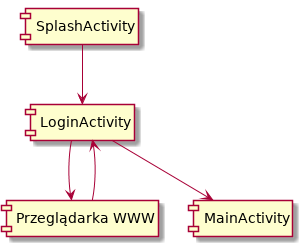
\includegraphics[scale=0.5]{img/activities.png}
\captionof{figure}{Aktywności aplikacji}\label{fig:activities}
\medskip
\endgroup

Najbardziej skomplikowaną aktywnością jest MainActivity. Składają się na nią
menu główne, belka tytułowa oraz wyświetlany ekran. Poszczególne ekrany w~obrębie
MainActivity są zrealizowane jako fragmenty (ang. \textit{fragment}). Przykładowo,
osobnymi fragmentami są: lista grup, lista protokołów, lista studentów w~konkretnym
terminie danego protokołu. Każdy fragment na własną rękę zajmuje się pobieraniem
danych z~USOS API, zapisywaniem ich w~pamięci tymczasowej (ang. \textit{cache}),
wyświetlaniem pobranych danych oraz obsługą interacji z~użytkownikiem. Dzięki temu,
że każdy fragment jest niezależny od danych pobranych przez inne fragmenty, informacje
wyświetlane na ekranie zawsze tworzą jedną spójną całość, a~zarządzanie danymi
składowanymi w~pamięci tymczasowej staje się bardzo proste. Na wygląd fragmentu mogą się
składać widoki (ang. \textit{view}), które reprezentują np. pojedyncze elementy
listy.

\section{Komunikacja z USOS API}

Każda uczelnia wdrażająca Mobilny USOS utrzymuje serwer USOS API, który dostarcza
aplikacji potrzebne dane. Dostęp do serwera jest broniony przez protokół
OAuth 1.0a \cite{oauth}. Cała komunikacja z~serwerem jest szyfrowana przy użyciu
protokołu TLS \cite{tls12}.

Każda aplikacja korzystająca z~serwera USOS API posiada własny klucz konsumenta
(ang. \textit{Consumer Key}). Służy on do identyfikacji aplikacji przez serwer
USOS API \cite{usosapi-auth}. Uczelnia kontroluje komu daje dostęp do USOS API
poprzez zgodę lub odmowę na wygenerowanie klucza. Klucze konsumenta dzielimy na
dwa rodzaje:
\begin{itemize}
	\item Zwykłe -- nie mają żadnych nadzwyczajnych uprawnień. Zazwyczaj
	pozwalają na pobieranie publicznie dostępnych danych lub działanie w~imieniu
	użytkownika, który wyraźnie się na to zgodził.
	\item Administracyjne -- przeznaczone są dla aplikacji zaufanych, takich jak
	aplikacje satelitarne USOS, np. USOSweb. W~zależności od uprawnień nadanych
	takiemu kluczowi, pozwala on na wykonywanie operacji bez wiedzy użytkownika
	oraz dostęp do wrażliwych danych.
\end{itemize}
Mobilny USOS jest publicznie dostępną aplikacją i~każda osoba może pobrać jej
plik wykonywalny, w~którym znajdują się klucze konsumenta. W~związku z~tym należy
liczyć się z~możliwością, że ktoś przy pomocy technik inżynierii wstecznej odczyta
jego klucz. Z~tego powodu nie wolno Mobilnemu USOS przydzielać administracyjnego
klucza konsumenta.

Każde zapytanie do USOS API odbywa się poprzez metodę POST protokołu HTTP.
Parametry zapytania są przekazywane w~identyczny sposób, w~jaki przesyłane są
pola formularza na stronie WWW. Każde zapytanie jest podpisane przy pomocy klucza
konsumenta i~tokenów użytkownika. Mobilny USOS otrzymuje tokeny użytkownika po
poprawnym zalogowaniu się osoby do USOS API. Aby utrudnić fałszowanie zapytań,
cześcią podpisu jest dokładny adres URL wywoływanej metody USOS API.

Opiszemy teraz ścieżkę, którą pokonuje typowe zapytanie do USOS API w~Mobilnym USOS.
Każda metoda USOS API ma swój opis w~kotlinowym interfejsie. Na ten opis składa
się sygnatura metody, pobierane parametry, nazwę klasy reprezentującej odpowiedź
serwera, typ żądania HTTP i~adres bazowy metody w~USOS API. Ten interfejs jest
przekazywany do biblioteki Retrofit, która generuje klasę wykonującą zapytanie i
obsługującą jego wynik. Retrofit jest skonfigurowany w~taki sposób, że przy
wywoływaniu kodu wykonującego zapytanie, jego parametry są przekazywane w~postaci
mapy klucz--wartość. Następnie zawartość tej mapy jest serializowana (o ile zachodzi
taka potrzeba), wyznaczany jest pełen adres URL wywoływanej metody na serwerze USOS
API i~tak gotowe zapytanie jest przekazywane do biblioteki OkHttp. Biblioteka
OkHttp dopisuje do zapytania nagłówki OAuth i~wysyła odpowiednie żądanie do serwera,
a następnie przekazuje odpowiedź do Retrofita. Odpowiedź serwera USOS API jest w
formacie JSON. Retrofit przy pomocy biblioteki Jackson dokonuje deserializacji
odpowiedzi, a~następnie wpisuje jej zawartość do kotlinowej klasy reprezentującej
zwrócony obiekt.

Komunikacja z~serwerem USOS API jest asynchroniczna. Moduł wykonujący zapytanie
do USOS API nie otrzymuje odpowiedzi wprost, ale w~postaci wywołania zwrotnego
(ang. \textit{callback}). Konieczność wykonania wielu zależnych od siebie zapytań
prowadzi do zjawiska znanego jako \textit{callback hell}. Wykonania poszczególnych
zapytań mogą ze sobą interferować, a~ich wyniki mogą być dostępne w~losowej kolejności.
Aplikacja musi śledzić, które zapytania się zakończyły, a~które jeszcze się wykonują.
Potrzebny staje się obiekt trzymający globalny stan. Dostęp do tego obiektu musi
być synchronizowany. Kod obsługujący wywołania staje się coraz dłuższy i~coraz
bardziej skomplikowany, a~notorycznie pojawiające się nieprzewidziane przeploty
powodują coraz częstsze błędy w~aplikacji. Zamiast skupić się na rozwoju nowej
funkcjonalności, programiści zmuszeni są poświęcać swój czas na tropienie i
naprawianie awarii.

Takie zjawiska miały miejsce, gdy przejęliśmy opiekę nad Mobilnym USOS. Był to
jeden z~najbardziej palących problemów. Rozwiązaliśmy go przy pomocy mechanizmu
korutyn zaimplementowanego w~języku Kotlin. Dzięki opakowaniu każdego wywołania
zwrotnego w~korutynę mogliśmy zapisać asynchroniczną logikę w~postaci synchronicznego
kodu. Uzyskaliśmy znaczne zmniejszenie rozmiaru kodu obsługującego komunikację z
USOS API, a~sam kod stał się znacznie czytelniejszy.

\section{Logowanie użytkownika do aplikacji}

Mobilny USOS jest traktowany przez USOS API jak aplikacja napisana przez niezależnego
programistę. Kiedy użytkownik chce się zalogować do aplikacji Mobilny USOS, to wysyła
do USOS API prośbę o~przydzielenie tymczasowych tokenów identyfikujących użytkownika
(ang. \textit{request token}). Do prośby dołączony jest adres wywołania zwrotnego,
na który po poprawnym zalogowaniu zostanie wysłany kod weryfikujący oraz lista
wymaganych przez aplikację uprawnień.

Następnie Mobilny USOS wywołuje kolejną metodę USOS API, która przekierowuje
użytkownika do ekranu logowania. To wywołanie ma miejsce w~przeglądarce zainstalowanej
w telefonie użytkownika. Dzięki temu użytkownik ma pewność, że Mobilny USOS nie
przechwytuje jego hasła do USOS. Ponadto może on ręcznie zweryfikować certyfikat SSL
by upewnić się, że łączy się z~prawdziwym serwerem USOS API. Gdybyśmy do realizacji
mechanizmu logowania wykorzystali komponent WebView osadzany wewnątrz aplikacji,
Mobilny USOS mógłby odczytać wszystkie dane wprowadzone na stronie logowania.
Ponadto użytkownik nie miałby możliwości zweryfikowania ważności certyfikatu SSL.
W związku z~tym twórcy USOS API odradzają podawanie swoich danych logowania w
aplikacji innej niż przeglądarka internetowa.

Poleganie na zewnętrznej aplikacji przysporzyło nam wielu problemów. Niektórzy
producenci telefonów zamiast przeglądarki będącej częścią projektu Android
dostarczają własne aplikacje. W~przypadku niektórych telefonów marki Samsung
okazało się, że taka przeglądarka niepoprawnie wyświetla stronę logowania, w
skutek czego użytkownik nie jest w~stanie zalogować się do USOS. Niektórzy
użytkownicy instalują własne przeglądarki, których konfiguracja nie pozwala na
poprawne działanie mechanizmu logowania. W~zależności od wersji systemu operacyjnego
istnieją rozbieżności między domyślnie instalowanymi przeglądarkami -- Android w
wersjach powyżej 5.0 korzysta z~Google Chrome, starsze wersje korzystają z~własnego
komponentu. Wszystko to sprawia, że nie da się uzyskać przewidywalnego środowiska,
w którym mógłby działać Mobilny USOS. Jednocześnie ze względu na mnogość różnych
konfiguracji nie jesteśmy w~stanie obsłużyć i~przetestować wszystkich możliwych
przypadków. Wykorzystanie zewnętrzej aplikacji ma jeszcze jedną wadę -- w~trakcie
testów użytkownicy narzekali, że po zakończonym procesie logowania w~tle pozostaje
otwarty proces przeglądarki, którego nie byliśmy w~stanie zamknąć. Czasem powodowało
to, że użytkownik w~panelu systemowym widział dwie otwarte aplikacje Mobilny USOS,
z czego poprawnie działała tylko jedna.

W obliczu wymienionych problemów zdecydowaliśmy się na następujące rozwiązanie.
Kiedy pojawia się potrzeba przekierowania użytkownika do przeglądarki, próbujemy
w pierwszej kolejności otworzyć Google Chrome. Jest to aplikacja sprawdzona,
poprawnie obsługująca stronę logowania do USOS oraz obecna na zdecydowanej
większości urządzeń. Ponadto obsługuje ona rozszerzenie Chrome Custom Tabs, które
pozwala nam osadzić przeglądarkę wewnątrz Mobilnego USOS. Taka przeglądarka w
dalszym ciągu zachowuje autonomię, która nie pozwala Mobilnemu USOS odczytać
hasła użytkownika, z~drugiej strony Mobilny USOS może lepiej kontrolować zachowanie
takiej przeglądarki. Jeżeli próba uruchomienia Google Chrome się nie powiedzie,
Mobilny USOS uruchamia domyślną przeglądarkę. Uważamy, że wypracowane rozwiązanie
jest dobrym kompromisem, dzięki któremu niemal wszyscy użytkownicy są w~stanie
zalogować się do Mobilnego USOS. Do tej pory nie otrzymaliśmy żadnej skargi na
działanie tego mechanizmu.

Po zalogowaniu USOS API przekierowuje użytkownika do wskazanego przez Mobilnego USOS
adresu URL. Wykorzystujemy mechanizm głębokiego linkowania (ang. \textit{deep links}),
by przekierować użytkownika z~przeglądarki z~powrotem do aplikacji \cite{deeplinks}.
W tym momencie do tymczasowych tokenów wygenerowanych wcześniej przez USOS API zostaje
przypisana tożsamość użytkownika. Mobilny USOS otrzymuje specjalny kod, który w
połączeniu z~tymczasowymi tokenami pozwala uzyskać od USOS API stałe tokeny (ang.
\textit{access token}), które są wykorzystywane w~dalszej komunikacji z~serwerem
USOS API.

\section{System obsługujący powiadomienia}

Większość pracy związanej z~obsługą powiadomień jest wykonywana przez usługę
Firebase Cloud Messaging, która odpowiada za transport powiadomienia z~serwera
USOS API do konkretnego urządzenia z~zainstalowanym Mobilnym USOS.
Na rysunku \ref{fig:messages} przedstawiony jest schemat integracji usług związanych z~obsługą powiadomień.

\begingroup
\centering
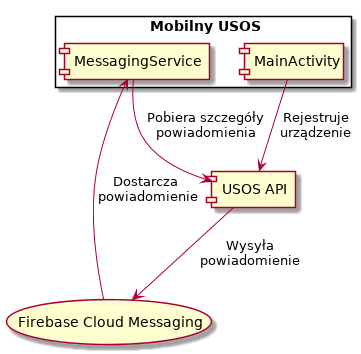
\includegraphics[scale=0.5]{img/messages.png}
\captionof{figure}{Usługi zaangażowane w~obsługę powiadomień}\label{fig:messages}
\medskip
\endgroup

Po zalogowaniu osoby do aplikacji, Firebase przydziela urządzeniu token, który
identyfikuje parę aplikacja--urządzenie. Ten token jest następnie wysyłany do
serwera USOS API, gdzie zostaje powiązany z~konkretnym użytkownikiem. Kiedy w~USOS
API zostanie wygenerowane nowe zdarzenie, takie jak pojawienie się nowej oceny,
zostaje ono wysłane do serwera Firebase Cloud Messaging. W~treści przesłanego
komunikatu znajduje się informacja, która pozwoli Mobilnemu USOS odtworzyć treść
zdarzenia oraz token urządzenia, do którego ma być wysłane powiadomienie. Nie
możemy w~treści komunikatu umieścić informacji, która byłaby uznana za daną osobową.
Z tego powodu dane przesyłane przez Firebase są stosunkowo mało szczegółowe. Po
otrzymaniu powiadomienia przez aplikację, Mobilny USOS pobiera z~serwera USOS API
brakujące informacje i~wyświetla je użytkownikowi. Proces wymiany danych między usługami
i~interakcje związane z~powiadomieniami są przedstawione na rysunku \ref{fig:firebase}.

\begingroup
\centering
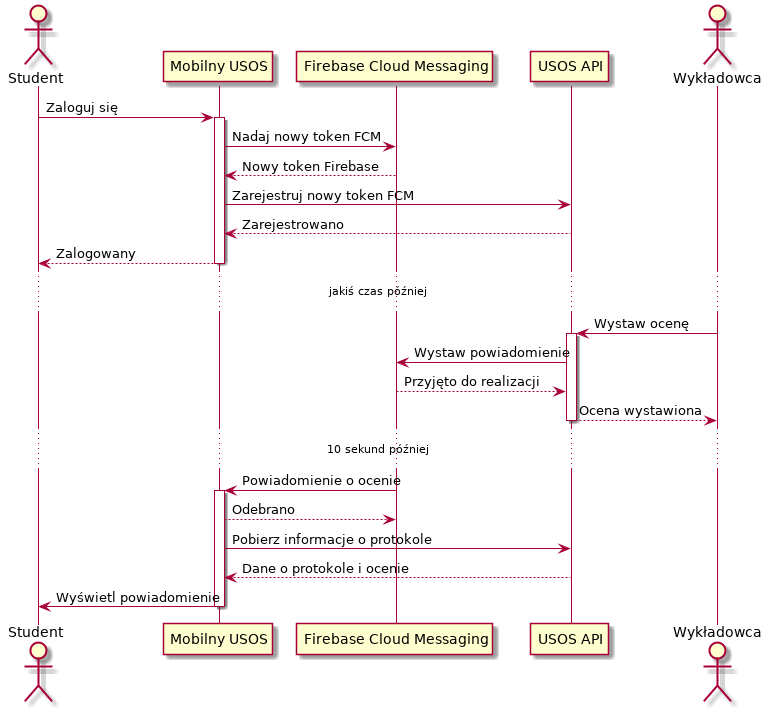
\includegraphics[scale=0.5]{img/firebase.png}
\captionof{figure}{Dostarczenie powiadomienia do użytkownika}\label{fig:firebase}
\medskip
\endgroup

Wielką uwagę przykładaliśmy do niezawodności mechanizmu powiadomień. Z~tego powodu
zdecydowaliśmy się na użycie gotowej, przetestowanej i~szeroko wykorzystywanej
usługi. Dzięki temu uniknęliśmy wielu problemów, które by się pojawiły gdybyśmy
sami podjęli się implementacji serwera powiadomień. Usługa odpowiedzialna za
odbieranie powiadomień jest cześcią systemu Android i~działa w~tle. Dzięki temu
Mobilny USOS otrzymuje powiadomienie nawet wtedy, gdy użytkownik wymusi zamknięcie
aplikacji. Dobra integracja z~ekosystemem Androida była kolejnym czynnikiem, który
przemawiał za wykorzystaniem Firebase.

Do Mobilnego USOS na jednym urządzeniu mogą być w~różnym czasie zalogowani różni
użytkownicy. W~sytuacji gdyby doszło do splotu kilku niekorzystnych okoliczności
związanych z~ograniczeniami serwera USOS API, mogłoby się zdarzyć, że do obecnie
zalogowanego użytkownika przyjdzie powiadomienie związane z~poprzednio zalogowanym
na urządzeniu użytkownkiem. Rozwiązujemy ten problem przez nieprzesyłanie danych
osobowych w~powiadomieniu, pomijanie powiadomień, gdy nikt nie jest zalogowany w
Mobilnym USOS na danym urządzeniu oraz przez wymuszenie wygenerowania nowego tokenu
Firebase po zalogowaniu nowego użytkownika. Dzięki temu zabiegowi nie grozi nam
sytuacja, kiedy na jeden token Firebase będą wysyłane powiadomienia dotyczące dwóch
różnych użytkowników.

\section{Budowa typowego fragmentu}

Podczas prac nad Mobilnym USOS szybko zauważyliśmy, że praktycznie wszystkie
fragmenty mają identyczny cykl życia. Po uruchomieniu fragmentu tworzone są
wszystkie jego komponenty graficzne. Następnie ekran jest zasłaniany przez pasek
ładowania i~w~tle inicjowane jest pobieranie danych z~USOS API. Równolegle fragment
próbuje odczytać dane zapisane w~pamięci urządzenia. Jeżeli mu się to uda, to
wyświetla wczytane dane i~usuwa pasek ładowania. W~międzyczasie z~USOS API mogą
zostać pobrane świeże dane. W~takiej sytuacji są one zapisywane do pamięci stałej,
a ekran jest odświeżany. Użytkownik może ręcznie zainicjować pobieranie danych z
serwera, aby odświeżyć wyświetlany widok. Jeżeli pobieranie danych się nie powiedzie,
trzeba wyświetlić odpowiedni komunikat o~błędzie.

Przedstawiony cykl życia jest stosunkowo skomplikowany, występuje w~nim wiele
przypadków brzegowych i~łatwo popełnić błąd podczas implementowania go. Z~tego
powodu postanowiliśmy wydzielić kod zarządzający cyklem życia fragmentu do osobnej
klasy bazowej. Każdy fragment dziedziczy po tej klasie i~implementuje interfejs,
zawierający metody obsługujące następujące żądania:

\begin{enumerate}
	\item Stwórz komponenty graficzne fragmentu.
	\item Pobierz dane z~USOS API.
	\item Wczytaj dane z~pamięci podręcznej.
	\item Zapisz dane w~pamięci podręcznej.
	\item Wyświetl odczytane lub pobrane dane.
\end{enumerate}

Wiele fragmentów w~Mobilnym USOS wyświetla listę obiektów, np. listę grup zajęciowych
albo listę protokołów. Stworzyliśmy klasę bazową, która zawiera kod wspólny takich
fragmentów. Dzięki temu programista nie musi za każdym razem implementować odpowiednich
widoków, filtrowania i~wyświetlania listy. Wystarczy, że zaimplementuje funkcje
odpowiedzialne za pobieranie danych z~USOS API i~tworzenie prostych struktur
opisujących pełną zawartość listy.

\section{Dostępność dla osób niepełnosprawnych}

Mobilny USOS musi spełniać wytyczne podane w~ustawie o~dostępności cyfrowej stron
internetowych i~aplikacji mobilnych podmiotów publicznych \cite{uodc}. Bazują one
na normach WCAG 2.1 \cite{wcag21}. Wiele spośród wymienionych norm Mobilny USOS
spełniał przed uchwaleniem ustawy, dlatego skupiliśmy się głównie na dostępności
dla osób niewidomych i~posiadających dysfunkcje narządu wzroku.

Podstawowym narzędziem systemu Android, z~którego korzystają osoby niewidome, jest
TalkBack. Służy on do głównie czytania zawartości ekranu i~nawigowania po systemie
przy pomocy gestów. Aby TalkBack działał poprawnie, wystarczyło w~Mobilnym USOS
dodać tekst alternatywny do obrazków. Możliwe jest zgrupowanie kilku elementów w
taki sposób, aby były czytane razem. Podmiana tekstu alternatywnego takiej grupy
pozwala sterować zawartością czytanego komunikatu. Skorzystaliśmy z~tej możliwości
w miejscach, gdzie czytanie pojedynczych elementów byłoby mylące lub czytanemu
elementowi brakowałoby kontekstu. Dobrym przykładem takiego miejsca jest ekran z
listą ocen, gdzie znaczenie poszczególnych pól tekstowych jest nadawane przez
graficzny układ elementów. Aby zapewnić odpowiednią dostępność, jako tekst alternatywny
ustawiliśmy słowny opis treści, którą chcieliśmy tym układem przekazać.

\section{Wymienność komponentów}

Jedną z~naszych decyzji projektowych było to, że każda uczelnia ma mieć własną
wersję aplikacji. Dzięki temu budowa Mobilnego USOS jest znacznie prostsza w~porównaniu
do sytuacji, gdy jedna aplikacja obsługuje wszystkie uczelnie, ale w~zamian za to
pojawia się wyzwanie związane z~utrzymywaniem wielu wersji aplikacji. W~związku z
tym zdecydowaliśmy, że uczelnie będą miały w~ograniczonym zakresie możliwość
personalizacji aplikacji. Więcej informacji na ten temat przedstawiliśmy w~rozdziale
poświęconym wdrożeniu.

\section{Szata graficzna}

Szata graficzna Mobilnego USOS jest ustandaryzowana. Poświęcamy bardzo wiele
uwagi jej spójności. Praktycznie wszystkie fragmenty są tworzone z~dwóch gotowych
szablonów. Użyte czcionki, rozmiary i~kolory tekstu, przycisków, grafik oraz odstępy
między elementami są jednolite. Sposób rozmieszczenia informacji na ekranie i
zastosowane ikonki są możliwie jak najbardziej spójne.

Jednym z~podstawowych elementów wyświetlanych na ekranie jest karteczka. Nazywamy
tak rzucający cień biały prostokąt z~zaokrąglonymi rogami. Służy on do wyświetlenia
podstawowej porcji informacji, takiej jak grupa na liście grup lub węzeł na liście
dzieci folderu sprawdzianu. Karteczka zazwyczaj składa się z~wyróżnionej informacji
głównej i~informacji pomocniczej zapisanej mniejszą czcionką. W~zależności od potrzeby
karteczka może być rozwijalna. Karteczki są najbardziej widocznym symbolem wysiłku
intelektualnego, jaki włożyliśmy w~to, by szata graficzna Mobilnego USOS była nie
tylko spójna, ale też elegancka.

Zezwalamy użytkownikom na częściową konfigurację wyglądu aplikacji. Do wyboru są
dwa motywy kolorystyczne -- domyślny jasny i~ciemny do użytku aplikacji w~nocy.
Ponadto użytkownik może niezależnie od ustawień systemowych ustawić sobie język
Mobilnego USOS, o~co prosiło nas wiele osób odbywających zagraniczne praktyki.

% coś o współpracy z grafikiem here

\chapter{Przegląd funkcjonalności}

% TODO dużo obrazków, trochę lania wody, dużo chwalenia się, że dowiezione rzeczy

\chapter{Wdrożenie w skali Polski}

Aplikację Mobilny USOS projektowaliśmy i~rozwijaliśmy z~myślą o~jej wdrażaniu we wszystkich zainteresowanych uczelniach
korzystających z~USOS. W~tym rozdziale przedstawimy wyzwania związane z~procesem wdrażania aplikacji Mobilny USOS na
polskich uczelniach.

\section{Wyzwania związane z wdrażaniem}

Podstawowym problemem, na który musieliśmy zwracać uwagę podczas projektowania i~wdrażania aplikacji, jest liczba
potencjalnie zainteresowanych uczelni -- obecnie 63 uczelnie należą do konsorcjum MUCI \cite{uczelnie-w-muci} i~każda
z~nich mogła być zainteresowana otrzymaniem aplikacji. W~okresie od października 2018 do lipca 2019 wdrożenia
produkcyjne zakończyło 14 uczelni \cite{news-musosumk, news-musospwste}, w~lipcu 2019 r. 7 kolejnych było w~fazie testów.

Liczba zainteresowanych zrodziła dwa główne problemy. Po pierwsze, poszczególne uczelnie mogą korzystać z~różnych
wersji USOS, w~szczególności USOS API. Należało więc utrzymać jednocześnie wsteczną zgodność na wypadek, gdyby uczelnie
nie aktualizowały systemu oraz dostarczać nowe funkcjonalności, które często wymagają nowej wersji USOS API. Drugim
problemem jest czas potrzebny na obsługę procesu wdrażania aplikacji do Google Play. Dodanie nowej wersji pakietu
wymaga od kilku do kilkunastu minut ręcznej pracy, co pomnożone przez liczbę uczelni mogłoby spowodować duże koszty
czasowe na proces aktualizacji.

\section{System budowania aplikacji}

Zdecydowaliśmy, że każda uczelnia otrzyma dedykowaną aplikację. Nazwy są budowane według schematu ,,Mobilny USOS'' i~skrócona nazwa uczelni, np. ,,Mobilny USOS UW''. 

W~ramach przygotowywania aplikacji, uczelnia ma dostarczyć:
\begin{enumerate}
	\item Dane dostępowe do USOS API -- adres serwera i~klucze autoryzacyjne.
	\item Klucze do integracji z~Google Firebase i~Google Maps.
	\item Logotyp uczelni oraz tło, które ma się pojawić w~menu. Dla przykładu, w~wersji dla Uniwersytetu Warszawskiego
        tłem jest zdjęcie Pałacu Kazimierzowskiego.
	\item Wzór nazwy uczelni do wyświetlenia na legitymacji studenckiej.
	\item (opcjonalnie) Wzór legitymacji pracowniczej -- zdjęcie pustej legitymacji i~układ tekstu oraz zdjęcia.
	\item (opcjonalnie) Sposób pobierania i~wyświetlania aktualności. Domyślnie moduł Aktualności pobiera dane z~USOS
        API i~wyświetla je poprzez uproszczone renderowanie HTML. Na życzenie uczelni możliwe jest wyświetlanie
        aktualności przez komponent \textit{WebView} \cite{webview}, choć nie jest to zalecane ze względu na istotny
        spadek wydajności aplikacji. Dostępna jest także integracja z~instalacją Wordpress uczelni i~pobieranie z~niej wiadomości.
	\item Klucz do podpisu aplikacji (na życzenie uczelni może być generowany po stronie MUCI).
	\item Adres strony z~polityką prywatności aplikacji ze względu na wymagania RODO. Uczelnie mogą skorzystać z~szablonu udostępnionego w~USOSweb.
	\item Adres e-mail do wysyłania powiadomień o~umieszczeniu na serwerze dystrybucyjnym nowej wersji aplikacji.
	\item Adres e-mail, który pojawi się pod przyciskiem ,,Napisz do nas'', służącym do kontaktu studentów i~pracowników z~działem wsparcia USOS na danej uczelni.
	\item (opcjonalnie) Lista modułów aplikacji, które mają zostać ukryte. Dla przykładu, jeśli
	uczelnia nie umieszcza w USOS planów zajęć, może chcieć usunąć z~aplikacji odpowiednią
	zakładkę.
\end{enumerate}

Z~perspektywy procesu budowania aplikacji każda uczelnia to osobny wariant aplikacji 
(\textit{product flavor} \cite{product-flavor}), w~którym umieszczone są dane dedykowane dla tej uczelni i~które w~trakcie
budowania są scalane z~kodem źródłowym wspólnym dla wszystkich. Dane wrażliwe, typu klucze autoryzacyjne i~hasła, są
umieszczone w~specjalnym pliku \texttt{private.gradle}, który nie jest wersjonowany w~repozytorium. Skonstruowany jest on
ponadto w~taki sposób, że dla skompilowania wersji dla danej uczelni, wymagany jest tylko wpis dla niej, dzięki czemu
możliwy jest rozwój aplikacji przez osoby z~różnych uczelni bez ryzyka pozyskania dostępu do cudzego systemu.

W~przypadku dodania do aplikacji nowej funkcjonalności, która wymaga nowszej wersji USOS API, sprawdzane jest przy starcie
aplikacji, czy uczelnia posiada odpowiednio aktualny system. Jeśli nie, funkcjonalność jest ukrywana przed użytkownikami.
Informujemy uczelnie o~konieczności aktualizacji serwera w~powiadomieniu o~nowej wersji i~w~dzienniku zmian.

Decyzja o~wydawaniu osobnych aplikacji zamiast jednej wspólnej pozwoliła także na przeniesienie na uczelnie obowiązku
utrzymania spójności wersji aplikacji i~USOS API. W~przypadku braku zgodności (na przykład gdyby zostały wprowadzone
wstecznie niekompatybilne zmiany w~aplikacji) aplikacja wyświetli komunikat z~prośbą o~kontakt z~uczelnią celem zaktualizowania
aplikacji lub serwera.

\section{Fabric i Crashlytics}

Istotną częścią procesu rozwoju aplikacji i~wdrażania na kolejne uczelnie były testy.

Do dystrybucji wersji testowych wykorzystaliśmy wspomniany wcześniej system Fabric \cite{fabric}. 
Integracja tego systemu z~Crashlytics pozwoliła nam na sprawne wykrywanie i~łatanie niedoskonałości w~aplikacji.

Dodatkowo przez Fabric udostępnialiśmy wersje deweloperskie aplikacji w~ramach specjalnej instancji DEMO. Dzięki temu
wszystkie osoby zainteresowane podglądem i~testami funkcjonalności aktualnie rozwijanych otrzymywały dedykowane wydania.
Dodatkowym czynnikiem, który przemawiał za użyciem Fabric jako systemu dystrybucji testowej była możliwość ustawienia grupy
docelowej dla każdego pakietu instalacyjnego z~osobna. Dzięki temu łatwo mogliśmy na przykład równolegle przedstawiać
Biuru Osób Niepełnosprawnych UW postępy w~zakresie dostosowywania aplikacji do potrzeb osób niepełnosprawnych, konsultować
z~grafikiem projekt graficzny modułu kalendarza i~testować edycję sprawdzianów przez pracownika.

\section{Jenkins}

W~związku z~decyzją, że każda uczelnia to inny wariant aplikacji, proces budowania nowej wersji oznaczał kompilowanie
kodu dla każdej uczelni osobno. Ponadto chcieliśmy, aby przygotowanie nowego wydania ograniczało się do kliknięcia przycisku
,,rozpocznij wdrożenie''. Należało także wybrać formę przekazywania skompilowanej aplikacji uczelniom, zgodnie
z~decyzją, że to uczelnie wybierają moment przeprowadzenia wdrożenia nowej wersji.

Skorzystaliśmy z~istniejącego systemu dystrybucji USOS i~narzędzia Jenkins. Zaletami tej decyzji są powszechne
wykorzystanie w~projekcie USOS, dzięki czemu wdrożeniowcy na uczelniach wiedzieli, jak odbierać od nas nowe wersje,
oraz wsparcie dla Jenkinsa wśród programistów USOS, także wśród tworzących Mobilnego USOS, ponieważ już we wczesnej
fazie rozwoju aplikacji była ona automatycznie testowana.

Jenkins dodatkowo przechowuje zależności i~szczegóły procesu budowania wewnątrz swojej konfiguracji, co istotnie
zmniejsza ryzyko awarii wywołanej niedopatrzeniem wdrożeniowca.

\section{Wdrożenie do sklepu Play}

Kolejnym z~efektów decyzji o~wydawaniu aplikacji dla każdej uczelni z~osobna była
konieczność opracowania procedury wdrażania aplikacji do sklepu Google Play w~taki
sposób, aby była jak najbardziej odporna na błędy ludzkie.

Dla wygody wdrażających i~dla maksymalnej spójności między uczelniami, stworzyliśmy
następujący schemat obsługi sklepu:
\begin{itemize}
	\item Dla każdej wersji aplikacji przygotowujemy krótkie podsumowanie zmian
	w~danej wersji po polsku i~angielsku.
	Uczelnia przekleja tę informację do pola ,,Co nowego'' w formularzu w~konsoli Google Play.
	\item Aplikacja ma ustandaryzowany opis funkcjonalności, uczelnia ma wyłącznie
	obowiązek wstawić do tego opisu swoją nazwę w~odpowiednim miejscu.
	\item Kolejne wersje aplikacji pojawiają się w~dedykowanym katalogu uczelni na
	serwerze z~dystrybucjami systemu USOS. Wdrażający pobiera odpowiedni plik i~bez
	modyfikacji umieszcza go w~konsoli. Google Play automatycznie wykryje i~wskaże
	wersję aplikacji.
	\item Na specjalny adres e-mail wysyłamy informację o~przygotowaniu nowej wersji
	aplikacji wraz z~odwołaniem do dziennika zmian i~informacją do sklepu. Ponadto,
	jeśli nowa wersja aplikacji zawiera moduł wymagający aktualizacji USOS API
	(o czym pisaliśmy wcześniej), zwracamy na to uwagę wdrażających zarówno w~dzienniku
	zmian, jak i~w~wiadomości.
\end{itemize}

Mechanizm ten sprawdził się dobrze w~praktyce, redukuje on do minimum potrzebną pracę
zarówno po stronie zespołu deweloperskiego, jak i~wdrażających na poszczególnych uczelniach.

\chapter{Podsumowanie}

Projekt Mobilny USOS jest naszym zdaniem dużym sukcesem. Udało nam się doprowadzić do
wdrożenia na wielu uczelniach aplikacji mobilnej dla systemu USOS, która posiadałaby
najważniejsze funkcje USOSweb w~użytecznej na telefonie formie.

W~kontekście sukcesu aplikacji istotnym wydaje się fakt, że wielu w powodzenie 
projektu nie wierzyło. Na Wydziale MIM UW chociażby gorzkim żartem przez wiele
lat było stwierdzenie, że co roku ktoś próbuje stworzyć aplikację mobilną dla USOS
i~co roku to nie wychodzi. Kilka takich projektów przez lata pojawiało się i~szybko
umierało z~braku zainteresowania studentów. 

Aplikacja została naszym zdaniem ciepło przyjęta przez studentów i~pracowników.
W~zależności od uczelni, oceny oscylują między 3.8 a~4.9 na 5 gwiazdek.
Wyjątkiem jest tu Uniwerystet Łódzki ze średnią ocen na poziomie 3.5/5, co prawdopodobnie
jest związane z~faktem, że na tej uczelni wdrożona została wersja przedprodukcyjna z~wieloma
błędami. Na pozostałych uczelniach większość negatywnych uwag była związana z~brakującymi
funkcjonalnościami, jak sprawdziany, więc wraz z~wdrażaniem nowych modułów, oceny powinny
wciąż rosnąć.

Duże plany wobec aplikacji ma Politechnika Warszawska. W~ramach ich projektu e-usług
aplikacja otrzyma kilka kolejnych modułów. W~międzyczasie
rozpoczął się port Mobilnego USOS na system iOS, jego pierwsza wersja została wdrożona
już m.in. na UW \cite{uw-ios, appstore}.

Aplikacja nie jest projektem zakończonym, czekamy na propozycje kolejnych przydatnych
funkcjonalności. W~ramach tej
pracy przygotowaliśmy bazę pod ciągłe rozbudowywanie i~ulepszanie komponentów aplikacji,
może to być na przykład tematem kolejnych prac magisterskich. Liczymy też w~dłuższej
perspektywie na to, że aplikacje wdrożą wszystkie uczelnie z~MUCI.

\appendix

\cleardoublepage
\phantomsection
\addcontentsline{toc}{chapter}{\listfigurename}
\listoffigures

\cleardoublepage
\phantomsection
\addcontentsline{toc}{chapter}{\listtablename}
\listoftables

% \nocite{*}

\begin{thebibliography}{99}
\addcontentsline{toc}{chapter}{Bibliografia}

%\bibitem[Bea65]{beaman} Juliusz Beaman, \textit{Morbidity of the Jolly
%   function}, Mathematica Absurdica, 117 (1965) 338--9.
%\bibitem[Ajax]{AJAXwikipl} AJAX - Wikipedia \url{https://pl.wikipedia.org/wiki/AJAX} (dostęp 21.03.2017)

\bibitem{euslugi} Uniwersytet Warszawski,
\textit{Rozwój e-usług Uniwersytetu Warszawskiego związanych z~edukacją},
\url{http://www.euslugi.uw.edu.pl/}. [Dostęp: 2019-07-24].

\bibitem{muci} Międzyuniwersyteckie Centrum Informatyzacji, Strona główna
\url{http://muci.edu.pl/index.html}. [Dostęp: 2019-07-24].

\bibitem{usos} Międzyuniwersyteckie Centrum Informatyzacji, \textit{USOS},
\url{https://www.usos.edu.pl/usos-start}. [Dostęp: 2019-07-24].

\bibitem{usosapi} Międzyuniwersyteckie Centrum Informatyzacji, \textit{USOS API Reference},
\url{https://apps.usos.edu.pl/developers/api/}. [Dostęp: 2019-07-24].

\bibitem{uodc} Sejm RP, \textit{Ustawa o~dostępności cyfrowej stron internetowych i~aplikacji mobilnych podmiotów publicznych}, Dz. U. z~2019~r., poz. 848.

\bibitem{talkback} Google Inc., \textit{TalkBack}, \url{https://support.google.com/accessibility/android/topic/3529932}. [Dostęp: 2019-05-07].

\bibitem{mifare} NXP Semiconductors Austria GmbH, \textit{Mifare ICs}, \url{https://www.mifare.net/en/products/chip-card-ics/}. [Dostęp: 2019-07-18].

\bibitem{mobywatel} Ministerstwo Cyfryzacji, \textit{mDokumenty. Potwierdzaj tożsamość smartfonem},\\ \url{https://obywatel.gov.pl/dokumenty-i-dane-osobowe/mdokumenty-potwierdzaj-tozsamosc-smartfonem}. [Dostęp: 2019-07-18].

\bibitem{wcag21} World Wide Web Consortium, \textit{Web Content Accessibility Guidelines (WCAG) 2.1},
\url{https://www.w3.org/TR/WCAG21/}. [Dostęp: 2019-06-17].

\bibitem{android} Google Inc., \textit{Android -- Documentation for app developers},
	 \url{https://developer.android.com/docs}. [Dostęp: 2019-05-04].

\bibitem{androidstudio} Google Inc., \textit{Android Studio},
	\url{https://developer.android.com/studio}. \\ 
	{[Dostęp: 2019-05-07]}.

\bibitem{androidsupportlibrary} Google Inc., \textit{Android -- Support Library},
	\url{https://developer.android.com/topic/libraries/support-library}. [Dostęp: 2019-05-07].

\bibitem{crashlytics} Google Inc., \textit{Crashlytics}, \url{https://try.crashlytics.com/}. [Dostęp: 2019-05-07].

\bibitem{fabric} Google Inc., \textit{Fabric}, \url{https://get.fabric.io/}. [Dostęp: 2019-05-07].

\bibitem{firebase} Google Inc., \textit{Firebase}, \url{https://firebase.google.com/}. [Dostęp: 2019-05-07].

\bibitem{firebasecm} Google Inc., \textit{Firebase Cloud Messaging},
	\url{https://firebase.google.com/docs/cloud-messaging}. [Dostęp: 2019-05-09].

\bibitem{git} Software Freedom Conservancy, \textit{Git},
	\url{https://git-scm.com/}. [Dostęp: 2019-05-07].

\bibitem{gerrit} Google Inc., \textit{Gerrit Code Review},
	\url{https://www.gerritcodereview.com/}.\\
	{[Dostęp: 2019-05-07]}.

\bibitem{jenkins} Continuous Delivery Foundation, \textit{Jenkins},
	\url{https://jenkins.io/}. [Dostęp: 2019-05-07].

\bibitem{gradle} Gradle Inc., \textit{Gradle}, \url{https://gradle.org/}. [Dostęp: 2019-05-07].

\bibitem{jackson} FasterXML, LLC., \textit{Jackson},
	\url{https://github.com/FasterXML/jackson}.\\
	{[Dostęp: 2019-05-07]}.

\bibitem{gson} Google Inc., \textit{Gson},	\url{https://github.com/google/gson}. [Dostęp: 2019-05-09].

\bibitem{java} Oracle Corporation, \textit{Java}, \url{https://www.java.com/}. [Dostęp: 2019-05-07].

\bibitem{kotlin} Kotlin Foundation, \textit{Kotlin}, \url{https://kotlinlang.org/}. [Dostęp: 2019-05-07].

\bibitem{kotlinandroid} Maxim Shafirov, \textit{Kotlin on Android. Now official},
	\url{https://blog.jetbrains.com/kotlin/2017/05/kotlin-on-android-now-official/}. [Dostęp: 2019-05-09].

\bibitem{okhttp} Square, Inc., \textit{OkHttp},	\url{https://square.github.io/okhttp/}. [Dostęp: 2019-05-07].

\bibitem{picasso} Square, Inc., \textit{Picasso}, \url{https://square.github.io/picasso/}. [Dostęp: 2019-05-07].

\bibitem{retrofit} Square, Inc., \textit{Retrofit}, \url{https://square.github.io/retrofit/}. [Dostęp: 2019-05-07].


\bibitem{googleplay} Google Inc., \textit{Google Play}, \url{https://play.google.com/store}. [Dostęp: 2019-05-07].

\bibitem{googlemaps} Google Inc., \textit{Google Maps},	\url{https://www.google.com/maps}. [Dostęp: 2019-05-07].

\bibitem{googlecalendar} Google Inc., \textit{Google Calendar},	\url{https://www.google.com/calendar}.\\
{[Dostęp: 2019-05-07]}.

\bibitem{gmail} Google Inc., \textit{Gmail}, \url{https://www.google.com/intl/pl/gmail/about/}.\\
{[Dostęp: 2019-05-07]}.

\bibitem{zxing} Google Inc., \textit{ZXing}, \url{https://github.com/zxing/zxing}. [Dostęp: 2019-05-07].

\bibitem{oauth} OAuth Core Workgroup, \textit{OAuth Core 1.0 Revision A}, \url{https://oauth.net/core/1.0a/}. [Dostęp: 2019-05-28].

\bibitem{tls12} Internet Engineering Task Force, \textit{The Transport Layer Security (TLS) Protocol}, \url{https://tools.ietf.org/html/rfc5246}. [Dostęp: 2019-05-28].

\bibitem{usosapi-auth} MUCI, \textit{USOS API Reference - Authorization}, \url{https://apps.usos.edu.pl/developers/api/authorization/}. [Dostęp: 2019-05-28].

\bibitem{deeplinks} Google Inc., \textit{Create Deep Links to App Content}, \url{https://developer.android.com/training/app-links/deep-linking}. [Dostęp: 2019-05-28].

\bibitem{uczelnie-w-muci} MUCI, \textit{Członkowie MUCI w~chronologicznej kolejności przystępowania do konsorcjum}, \url{https://www.usos.edu.pl/czlonkowie-muci-w-chronologicznej-kolejnosci-przystepowania-do-konsorcjum}. [Dostęp: 2019-05-20].

\bibitem{news-musosumk} MUCI, \textit{Mobilny USOS UMK w~sklepie Google Play}, \url{https://www.usos.edu.pl/node/4157/mobilny-usos-umk-w-sklepie-google-play}. [Dostęp: 2019-05-20].

\bibitem{news-musospwste} MUCI, \textit{Mobilny USOS PWSTE w~sklepie Google Play}, \url{https://www.usos.edu.pl/node/4170/mobilny-usos-pwste-w-sklepie-google-play}. [Dostęp: 2019-07-19].

\bibitem{webview} Google Inc., \textit{WebView}, \url{https://developer.android.com/reference/android/webkit/WebView}. [Dostęp: 2019-05-20].

\bibitem{product-flavor} Google Inc., \textit{Configure build variants}, \url{https://developer.android.com/studio/build/build-variants#product-flavors}. [Dostęp: 2019-05-20].

\bibitem{uw-ios} Uniwersytet Warszawski,
\textit{Aplikacja Mobilny USOS już dostępna na iOS},\\
\url{https://www.uw.edu.pl/aplikacja-mobilny-usos-juz-dostepna-na-ios/}.\\
{[Dostęp: 2019-07-18]}.

\bibitem{appstore} Apple Inc.,
\textit{Aplikacja Mobile USOS UW w~App Store},\\
\url{https://apps.apple.com/us/app/mobilny-usos-uw/id1447221710}.\\
{[Dostęp: 2019-07-18]}.

\end{thebibliography}

\end{document}


%%% Local Variables:
%%% mode: latex
%%% TeX-master: t
%%% coding: latin-2
%%% End:
